\documentclass{article}
\usepackage{xcolor}
\usepackage{amsmath,amssymb}
\usepackage{pagecolor}
\usepackage{lipsum}
\usepackage{fullpage}
\usepackage{tikz}

\newcommand{\magn}[1]{\left\Vert #1 \right\Vert}
\newcommand{\bkt}[1]{\left(#1\right)}
\newcommand{\Rb}{\mathbb{R}}
\newcommand{\dsum}{\displaystyle\sum}
\newcommand{\cntr}[1]{\begin{center}#1\end{center}\vspace{1em}}
\pagecolor{black}
\color{white}

\begin{document}
	\large
	\begin{center}
	\emph{For any} $X \in \Rb^{n \times n}$ and $\epsilon \in (0,1]$. Then, with $r= \left\lceil 72\log(2n+1)/\epsilon^2\right\rceil$, we have
	$$\inf_{\text{rank}\bkt{Y} \leq r} \magn{X-Y}_{\max} \leq \epsilon \magn{X}_2$$
	\end{center}
	\newpage
	\begin{center}
		$$\begin{bmatrix}
		\color{red}{1} & \color{orange}{2} & \color{white}{3} & \color{green}{4} & \color{cyan}{5}\\
		\color{cyan}{5} & \color{red}{1} & \color{orange}{2} & \color{white}{3} & \color{green}{4}\\
		\color{green}{4} & \color{cyan}{5} & \color{red}{1} & \color{orange}{2} & \color{white}{3}\\
		\color{white}{3} & \color{green}{4} & \color{cyan}{5} & \color{red}{1} & \color{orange}{2}\\
		\color{orange}{2} & \color{white}{3} & \color{green}{4} & \color{cyan}{5} & \color{red}{1}\\
		\end{bmatrix}$$
	\end{center}
	\newpage
	
	\LARGE
	\cntr{$N$ charges: $\{q_i,r_i\}_{i=1}^N$}
	\cntr{Potential: $\phi_i = \dsum_{j \neq i} \dfrac{q_j}{\magn{r_i-r_j}}$ for $i \in \{1,2,\ldots,N\}$}
	\cntr{Note that we have $\phi = Aq$, $\phi$ is the set of potentials, $q$ is the set of charges and $A_{ij} = \dfrac1{\magn{r_i-r_j}}$ for $i \neq j$}
	\cntr{Matrix-vector product: Given $q$, compute $\phi$. Cost is $\mathcal{O}(N^2)$}
	\cntr{Solve linear system: Given $\phi$, compute $q$. Cost is $\mathcal{O}(N^3)$}
	\cntr{Can we reduce the above computational complexity to say $\mathcal{O}(N)$?}
	
	\newpage
	\LARGE
	\cntr{Let's look at a slightly easier problem}
	\cntr{$N$ charges: $\{q_i,r_i\}_{i=1}^N$}
	\cntr{Potential: $\phi_i = \dsum_{j=1}^N \sin\bkt{k \bkt{r_i - r_j}} q_j$ for $i \in \{1,2,\ldots,N\}$}
	\cntr{Matrix-vector product: $Aq$, where $A_{ij} =\sin\bkt{k \bkt{r_i - r_j}}$ for $i \neq j$}
	\cntr{Computational cost is $\mathcal{O}(N^2)$}
	\cntr{Can we reduce the computational complexity?}
	\newpage
	\cntr{Note that $\sin\bkt{k \bkt{r_i - r_j}} = \sin\bkt{k r_i} \cos\bkt{k r_j} - \cos\bkt{k r_i} \sin\bkt{k r_j}$}
	\cntr{$$\phi_i = \dsum_{j=1}^N \sin\bkt{k r_i} \cos\bkt{k r_j} q_j - \dsum_{j=1}^N \cos\bkt{k r_i} \sin\bkt{k r_j} q_j$$
	for $i \in \{1,2,\ldots,N\}$}
	\cntr{$$\phi_i = \bkt{\dsum_{j=1}^N\cos\bkt{k r_j} q_j}\sin\bkt{k r_i}  - \bkt{\dsum_{j=1}^N \sin\bkt{k r_j} q_j}\cos\bkt{k r_i} $$
	for $i \in \{1,2,\ldots,N\}$}
	\cntr{Compute $a = \dsum_{j=1}^N\cos\bkt{k r_j} q_j$; Cost is $\mathcal{O}(N)$}
	\cntr{Compute $b = \dsum_{j=1}^N\sin\bkt{k r_j} q_j$; Cost is $\mathcal{O}(N)$}
	\cntr{$\phi_i = a \sin\bkt{kr_i} - b \cos\bkt{kr_i}$ for $i \in \{1,2,\ldots,N\}$; Cost is $\mathcal{O}(N)$}
	\cntr{Total cost is $\mathcal{O}(N)$}
	\cntr{Wait... What happened?}
	\cntr{How did we go from $\mathcal{O}(N^2)$ to $\mathcal{O}(N)$?}
	\cntr{In matrix form, we rewrote the matrix $A$ as}
	$$A = u_1 v_1^T - v_1 u_1^T$$
	$$A = \begin{bmatrix}
	u_1 & -v_1
	\end{bmatrix}_{N \times 2}
	\begin{bmatrix}
		v_1^T\\
		u_1^T
	\end{bmatrix}_{2 \times N}
	$$
	$$u_1 = \begin{bmatrix}
	\sin\bkt{kr_1}\\
	\sin\bkt{kr_2}\\
	\vdots\\
	\sin\bkt{kr_N}\\
	\end{bmatrix}$$
	$$v_1 = \begin{bmatrix}
	\cos\bkt{kr_1}\\
	\cos\bkt{kr_2}\\
	\vdots\\
	\cos\bkt{kr_N}\\
	\end{bmatrix}$$
	Hence,
	$$Aq = u_1 \bkt{v_1^Tq} - v_1 \bkt{u_1^Tq}$$
	
	\newpage
	

	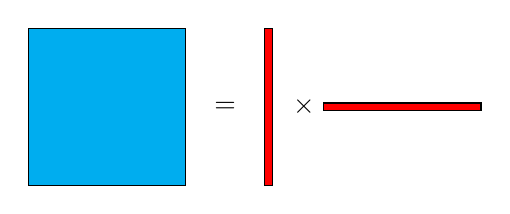
\begin{tikzpicture}
	\draw[fill=cyan] (0,0) rectangle (2,2);
	\path (2.5,1) node (=) {$=$};
	\draw[fill=red] (3,0) rectangle (3.1,2);
	\path (3.5,1) node (times) {$\times$};
	\draw[fill=red] (3.75,0.95) rectangle (5.75,1.05);
	% \path (5.75,1) node (where) {; where};
	% \draw[fill=cyan] (6.75,1.4) rectangle (6.95,1.6);
	% \draw[->] (7,1.5) -- (7.25,1.5);
	% \draw[fill=red] (6.75,0.4) rectangle (6.95,0.6);
	% \draw[->] (7,0.5) -- (7.25,0.5);
	% \path (8.6,1.5) node(lowrank) {Low-rank matrix};
	% \path (8.6,0.5) node(fullrank) {Full-rank matrix};
	\end{tikzpicture}
	
	\newpage

	\begin{center}
	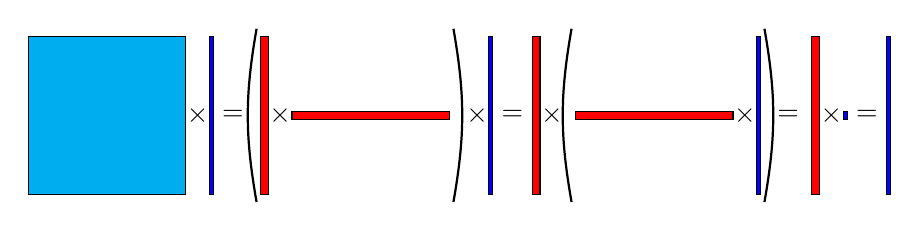
\begin{tikzpicture}
	\draw[fill=cyan] (0,0) rectangle (2,2);
	\path (2.15,1) node (times) {$\times$};
	\draw[fill=blue] (2.3,0) rectangle (2.35,2);
	\path (2.6,1) node (=) {$=$};

	\draw[thick] (2.9,2.1) to [out=260, in=100] (2.9,-0.1);
	\draw[fill=red] (2.95,0) rectangle (3.05,2);
	\path (3.2,1) node (times) {$\times$};
	\draw[fill=red] (3.35,0.95) rectangle (5.35,1.05);
	\draw[thick] (5.4,2.1) to [out=280, in=80] (5.4,-0.1);
	\path (5.7,1) node (times) {$\times$};
	\draw[fill=blue] (5.85,0) rectangle (5.9,2);

	\path (6.15,1) node (=) {$=$};
	\draw[fill=red] (6.4,0) rectangle (6.5,2);
	\path (6.65,1) node (times) {$\times$};
	\draw[thick] (6.9,2.1) to [out=260, in=100] (6.9,-0.1);
	\draw[fill=red] (6.95,0.95) rectangle (8.95,1.05);
	\path (9.1,1) node (times) {$\times$};
	\draw[fill=blue] (9.25,0) rectangle (9.3,2);
	\draw[thick] (9.35,2.1) to [out=280, in=80] (9.35,-0.1);

	\path (9.65,1) node (=) {$=$};
	\draw[fill=red] (9.95,0) rectangle (10.05,2);
	\path (10.2,1) node (times) {$\times$};
	\draw[fill=blue] (10.35,0.95) rectangle (10.4,1.05);

	\path (10.65,1) node (=) {$=$};
	\draw[fill=blue] (10.9,0) rectangle (10.95,2);
	\end{tikzpicture}
	\end{center}
	
	\newpage
	\cntr{Does the same idea work for $1/\magn{r_i-r_j}$ instead of $\sin\bkt{k\bkt{r_i-r_j}}$?}
	\cntr{Unfortunately, not.}
	\cntr{The ``kernel" (Green's function) $1/r$ has a singularity at the origin.}
	\cntr{Let's look at other kernel functions; For instance, $\log(r)$}
	\cntr{But what about away from the singularity?}
	\cntr{Away from the singularity the matrix looks like low-rank (?)}
	\cntr{Can this be proved?}
	\cntr{Yes! The matrix is indeed low-rank in finite precision!}
	\cntr{Away from the singularity, the kernel is smooth and a separable expansion of the kernel can be obtained}
	\cntr{
	$$K\bkt{x,y} = \dsum_{i,j=1}^r c_{ij} \phi_i(x) \psi_j(y) + \mathcal{O}\bkt{\epsilon}$$
	where $r = \mathcal{O}\bkt{\log\bkt{1/\epsilon}}$ uniformly across the domain of $x$ and $y$.
	}
	\cntr{An appropriate series (Taylor or Eigen-function) expansion of the kernel into separable expansions}
	\cntr{We could also rely on polynomial interpolation to construct separable expansions}
	\cntr{The rank $r$ is {\color{green}\emph{independent}} of $N$}
	

	
	\newpage
	\cntr{Fast Multipole Method - souped version of the previous mentioned}
	
	\begin{itemize}
		\item Relies on hierarchically sub-dividing your domain
		\item Identifying blocks to leverage low-rank matrix vector products
	\end{itemize}

	\cntr{Total computational complexity is $\mathcal{O}(r N)$}
	
	\cntr{Fast Multipole Method in Computational Physics}
	
	\cntr{Matrices arising out of N-body problems have an even nicer structure}
\end{document}